\section{Acerca del Autor}

\begin{figure}[h]
\begin{minipage}{11.5cm}

\subsection{Reseña}

Leo Soto es Ingeniero Informático de la USACH, socio de Continuum y
desarrollador para Hashrocket Chile. Se define como un programador políglota, y
disfruta aprendiendo nuevos lenguajes de programación para agregar a su caja de
herramientas. Ha desarrollado profesionalmente en C, C\#, Java, Scala, Python,
Ruby, PHP, Javascript y Flex y maneja también otros lenguajes como Erlang,
Objective-C y Lisp.

Ha dictado charlas fuera del país en la DjangoCon 2008 realizada en el
GooglePlex en Mountain View, y en la PyCon 2009 en Chicago. En el medio nacional
ha participado como expositor en las FLISOL 2009 y 2010, Encuentro Linux 2008 y
2009 y en las Jornadas Regionales del Software Libre 2009.

\end{minipage}
\begin{minipage}{1.7in}
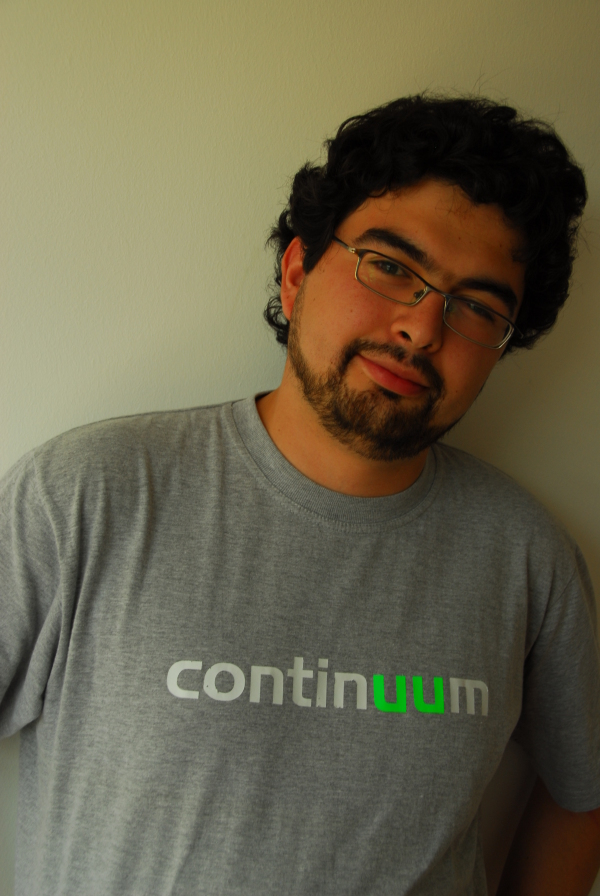
\includegraphics[width=1.5in]{images/foto.jpg}
\end{minipage}
\end{figure}

\subsection{Datos de contacto}

\begin{itemize}
\item{\textbf{E-mail:} leo.soto@gmail.com}
\item\textbf{{Teléfono:} 9 8733 9008}
\item{\textbf{URL:} \url{http://blog.leosoto.com}}
\end{itemize}
